\documentclass[table,xcolor=dvipsnames,professionalfonts]{beamer}
\usepackage{xcolor}
\usepackage{booktabs}
\usepackage{graphicx}
\usepackage{tikz}
\usepackage{feynmp}
\usepackage{xspace}
\usepackage{slashed}
%\usepackage[utopia]{mathdesign}
\usepackage[charter]{mathdesign}
\usepackage[UKenglish]{babel}
\usepackage[utf8]{inputenc}
%\usepackage{lmodern}
\setbeamertemplate{navigation symbols}{}
\usepackage{appendixnumberbeamer}
%\usepackage{hepparticles}
%\usepackage{hepnicenames}
\usepackage{hepunits}
\usepackage{bbm}

\ifpdf
\usepackage{epstopdf}
\usepackage[protrusion=true,expansion=true,tracking]{microtype}
%\DeclareGraphicsRule{*}{mps}{*}{}
\fi

\usepackage{listings}
\usepackage[framemethod=tikz]{mdframed}
\lstloadlanguages{C++}
\makeatletter
\newcommand{\srcsize}{\@setfontsize{\srcsize}{5pt}{5pt}}
\makeatother
\lstset{language=[11]C++,
  literate= % define some ligatures for PragmataPro
  {!!}{\texttt{!!}}2 {::}{\texttt{::}}2 {++}{\texttt{++}}2
  {--}{\texttt{--}}2 {()}{\texttt{()}}2 {\[\]}{\texttt{[]}}2
  {==}{\texttt{==}}2 {!=}{\texttt{!=}}2 {>=}{\texttt{>=}}2
  {<=}{\texttt{<=}}2 {&&}{\texttt{\&\&}}2 {||}{\texttt{||}}2
  {!>}{\texttt{!>}}2 {\#(}{\texttt{\#(}}2 {\#_}{\texttt{\#_}}2
  {\#\{}{\texttt{\#\{}}2 {\#?}{\texttt{\#?}}2 {\#>}{\texttt{\#>}}2
  {\%=}{\texttt{\%=}}2 {+=}{\texttt{+=}}2 {-=}{\texttt{-=}}2
  {*=}{\texttt{*=}}2 {/=}{\texttt{/=}}2 {&=}{\texttt{&=}}2
  {^=}{\texttt{^=}}2 {|=}{\texttt{|=}}2 {~=}{\texttt{~=}}2
  {<<}{\texttt{<<}}2 {>>}{\texttt{>>}}2 {->}{\texttt{->}}2
  {__}{\texttt{\_\_}}2
  {!!!}{\texttt{!!!}}3 {>>=}{\texttt{>>=}}3 {<<=}{\texttt{<<=}}3
  {/==}{\texttt{/==}}3 {...}{\texttt{...}}3,
  deletekeywords=[1]{auto,const,static,volatile,void,char,short,int,long,unsigned,float,double,inline,template,typename,namespace,class,union,struct,enum,true,false,nullptr},
  morekeywords=[2]{auto,const,static,volatile},
  morekeywords=[3]{void,char,short,int,long,unsigned,float,double,size_type,inline,iterator,const_iterator,reference,const_reference,Uninitialised,template,typename,namespace,class,union,struct,enum},
  morekeywords=[4]{std,our,LHCb,T,ARGS},
  morekeywords=[5]{true,false,nullptr,__LINE__,__FILE__,__func__},
  basicstyle=\srcsize\ttfamily\color{black},
  keywordstyle=[1]\color{magenta}\textbf,
  keywordstyle=[2]\color{orange}\textbf,
  keywordstyle=[3]\color{cyan}\textbf,
  keywordstyle=[4]\color{black},
  keywordstyle=[5]\color{violet!80!white},
  directivestyle=\color{blue!50!white},
  commentstyle=\color{blue}\textsl,
  stringstyle=\color{gray},
  identifierstyle=\color{green!50!black},
breaklines=true,breakautoindent=true}

\mdfdefinestyle{listing}{
  backgroundcolor=white!96!black,hidealllines,
  skipabove=0pt,skipbelow=0pt,
  leftmargin=0pt,rightmargin=0pt,
  innertopmargin=-5pt,innerbottommargin=-5pt,
  innerleftmargin=0pt,innerrightmargin=0pt,
  linewidth=0pt,middlelinewidth=0pt,
  startcode={\vspace{-3pt}},endcode={\vspace{-2ex}}
}
\surroundwithmdframed[style=listing]{lstlisting}

\usepackage{fontspec}
%\setmainfont{CharisSIL}[]
%\setsansfont{FrontPagePro}[Scale=MatchLowercase]

\def\shrug{\texttt{\raisebox{0.75em}{\char`\_}\char`\\\char`\_\kern-0.5ex(\kern-0.25ex\raisebox{0.25ex}{\rotatebox{45}{\raisebox{-.75ex}"\kern-1.5ex\rotatebox{-90})}}\kern-0.5ex)\kern-0.5ex\char`\_/\raisebox{0.75em}{\char`\_}}}

\usetheme{Rochester}
%\usecolortheme{beaver}
\usecolortheme[named=NavyBlue]{structure}
\setbeamercolor{section in toc}{fg=black,bg=white}
%\setbeamercolor{alerted text}{fg=blue}
\setbeamercolor{structure}{fg=blue!80!black}
\setbeamercolor*{palette primary}{fg=black,bg=gray!30!white}
\setbeamercolor*{palette secondary}{fg=black,bg=gray!15!white}
\setbeamercolor*{palette tertiary}{bg=blue!80!black,fg=gray!10!white}
\setbeamercolor*{palette quaternary}{fg=blue,bg=gray!5!white}
\setbeamercolor*{sidebar}{fg=blue,bg=gray!15!white}
\setbeamercolor*{palette sidebar primary}{fg=blue!10!black}
\setbeamercolor*{palette sidebar secondary}{fg=white}
\setbeamercolor*{palette sidebar tertiary}{fg=blue!50!black}
\setbeamercolor*{palette sidebar quaternary}{fg=gray!10!white}
\setbeamercolor{titlelike}{parent=palette primary,fg=blue,bg=white}
\setbeamercolor{frametitle}{fg=white,bg=blue!80!black}
\setbeamercolor{frametitle right}{bg=gray!60!white}
\setbeamercolor*{separation line}{}
\setbeamercolor*{fine separation line}{}
\useinnertheme{rectangles}
\useoutertheme{infolines}
\usefonttheme[onlymath]{serif}
%\usefonttheme{professionalfonts}


\setbeamertemplate{footline}
{
  \leavevmode%
  \hbox{%
    \begin{beamercolorbox}[wd=.333333\paperwidth,ht=2.25ex,dp=1ex,left]{author in head/foot}%
      \usebeamerfont{author in head/foot}%
      \hfill \insertshortauthor \hfill%
    \end{beamercolorbox}%
    \begin{beamercolorbox}[wd=.333333\paperwidth,ht=2.25ex,dp=1ex,center]{title in head/foot}%
      \usebeamerfont{title in head/foot}\insertshorttitle%
    \end{beamercolorbox}%
    \begin{beamercolorbox}[wd=.333333\paperwidth,ht=2.25ex,dp=1ex,right]{date in head/foot}%
      \usebeamerfont{date in head/foot}\insertshortdate{}\hspace*{2em}%
      42 / 42 \hspace*{2ex} %
    \end{beamercolorbox}%
  }%
  \vskip0pt%
}

\setbeamertemplate{frametitle}
{
  \ifbeamercolorempty[bg]{frametitle}{}{\nointerlineskip}%
  \leavevmode%
  \vskip-2pt\hbox{%
    \begin{beamercolorbox}[wd=\paperwidth,left]{frametitle}%
      \usebeamerfont{frametitle}%
      \vskip.125ex%
      \hbox{\vtop{\raisebox{-1ex}[1ex][1ex]{}%
      \hspace{1em}\strut\insertframetitle\strut}\par%
      {%
        \ifx\insertframesubtitle\@empty%
        \else%
        {\usebeamerfont{framesubtitle}\usebeamercolor[fg]{framesubtitle}\insertframesubtitle\strut\par}%
        \fi
      }}%
    \end{beamercolorbox}%
  }%
}


\definecolor{bandgreen}{rgb}{0.4,0.8,0.4}
\newcommand{\FIXME}{{\color{red}FIXME}}
\newcommand{\arxiv}[1]{{\color{gray}\tiny$[$\href{http://arxiv.org/abs/#1}{arXiv:#1}$]$}}
\newcommand{\jref}[2]{{\color{gray}\tiny$[$\href{#2}{#1}$]$}}
\newcommand{\myhref}[2]{\href{#1}{\textcolor{red}{#2}}}


\author[Paul]{pseyfert}
\institute[]{
\includegraphics[width=.25\textwidth]{./QR.png}}
\date[]{}
\title[use your garmin without garmin's cloud]{{use your garmin without garmin's cloud}\newline \myhref{https://github.com/pseyfert/fitfile-jugglers}{https://github.com/pseyfert/fitfile-jugglers}}
  \AtBeginSection[]
  {
    %\beamertemplateshadingbackground{Red!30!White}{White}
    \begin{frame}<beamer>{}
      %\tableofcontents[currentsection,currentsubsection]
      \tableofcontents[currentsection]
    \end{frame}
    %\beamertemplateshadingbackground{Red!01!White}{White}
  }


\begin{document}
\maketitle

\section{initial problem}
\subsection{}
\begin{frame}
  \frametitle{}
  I have a Garmin sports watch
  \begin{exampleblock}{design}
    Sync watch with smartphone to the cloud and let garmin harvest data and watch result in the webbrowser
  \end{exampleblock}
  \begin{alertblock}{what i want}
    \begin{itemize}
        \item have analysis fun myself!
        \item have analysis fun even on bad wifi
        \item have data for my eyes only
    \end{itemize}
  \end{alertblock}
%  I have a Garmin sports watch and I can download gpx files from the Garmin connect webpage but there are a few things wrong with it
%  \begin{itemize}
%    \item I want to nerd around with the data it records even if no GPS is available
%    \item I want to convert a month of data into data formats I understand w/o clicking hundreds of download buttons on the garmin webpage
%    \item I often have crappy internet and don't want to go mental while data sloooooowly goes from my wrist to my phone to the cloud and back onto my lap
%  \end{itemize}
%  \begin{alertblock}{}
%    \begin{itemize}
%      \item will Garmin sell my data to my health insurance?
%      \item will my co-workers ever see that I don't work on their tickets but walk around?
%      \item will my employer ever see that I sleep at work and do hiking tours at night?
%      \item how do I ensure Garmin doesn't get hacked?
%    \end{itemize}
%  \end{alertblock}
\end{frame}

\section{solution}
\begin{frame}
  \frametitle{modus operandi}
  \begin{itemize}
    \item device needs charging anyway
    \item automounts w/o problem (on home user linux)
  \end{itemize}
  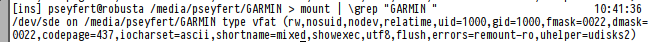
\includegraphics[width=\textwidth]{./mount.png}
  \begin{columns}
    \begin{column}{.5\textwidth}
      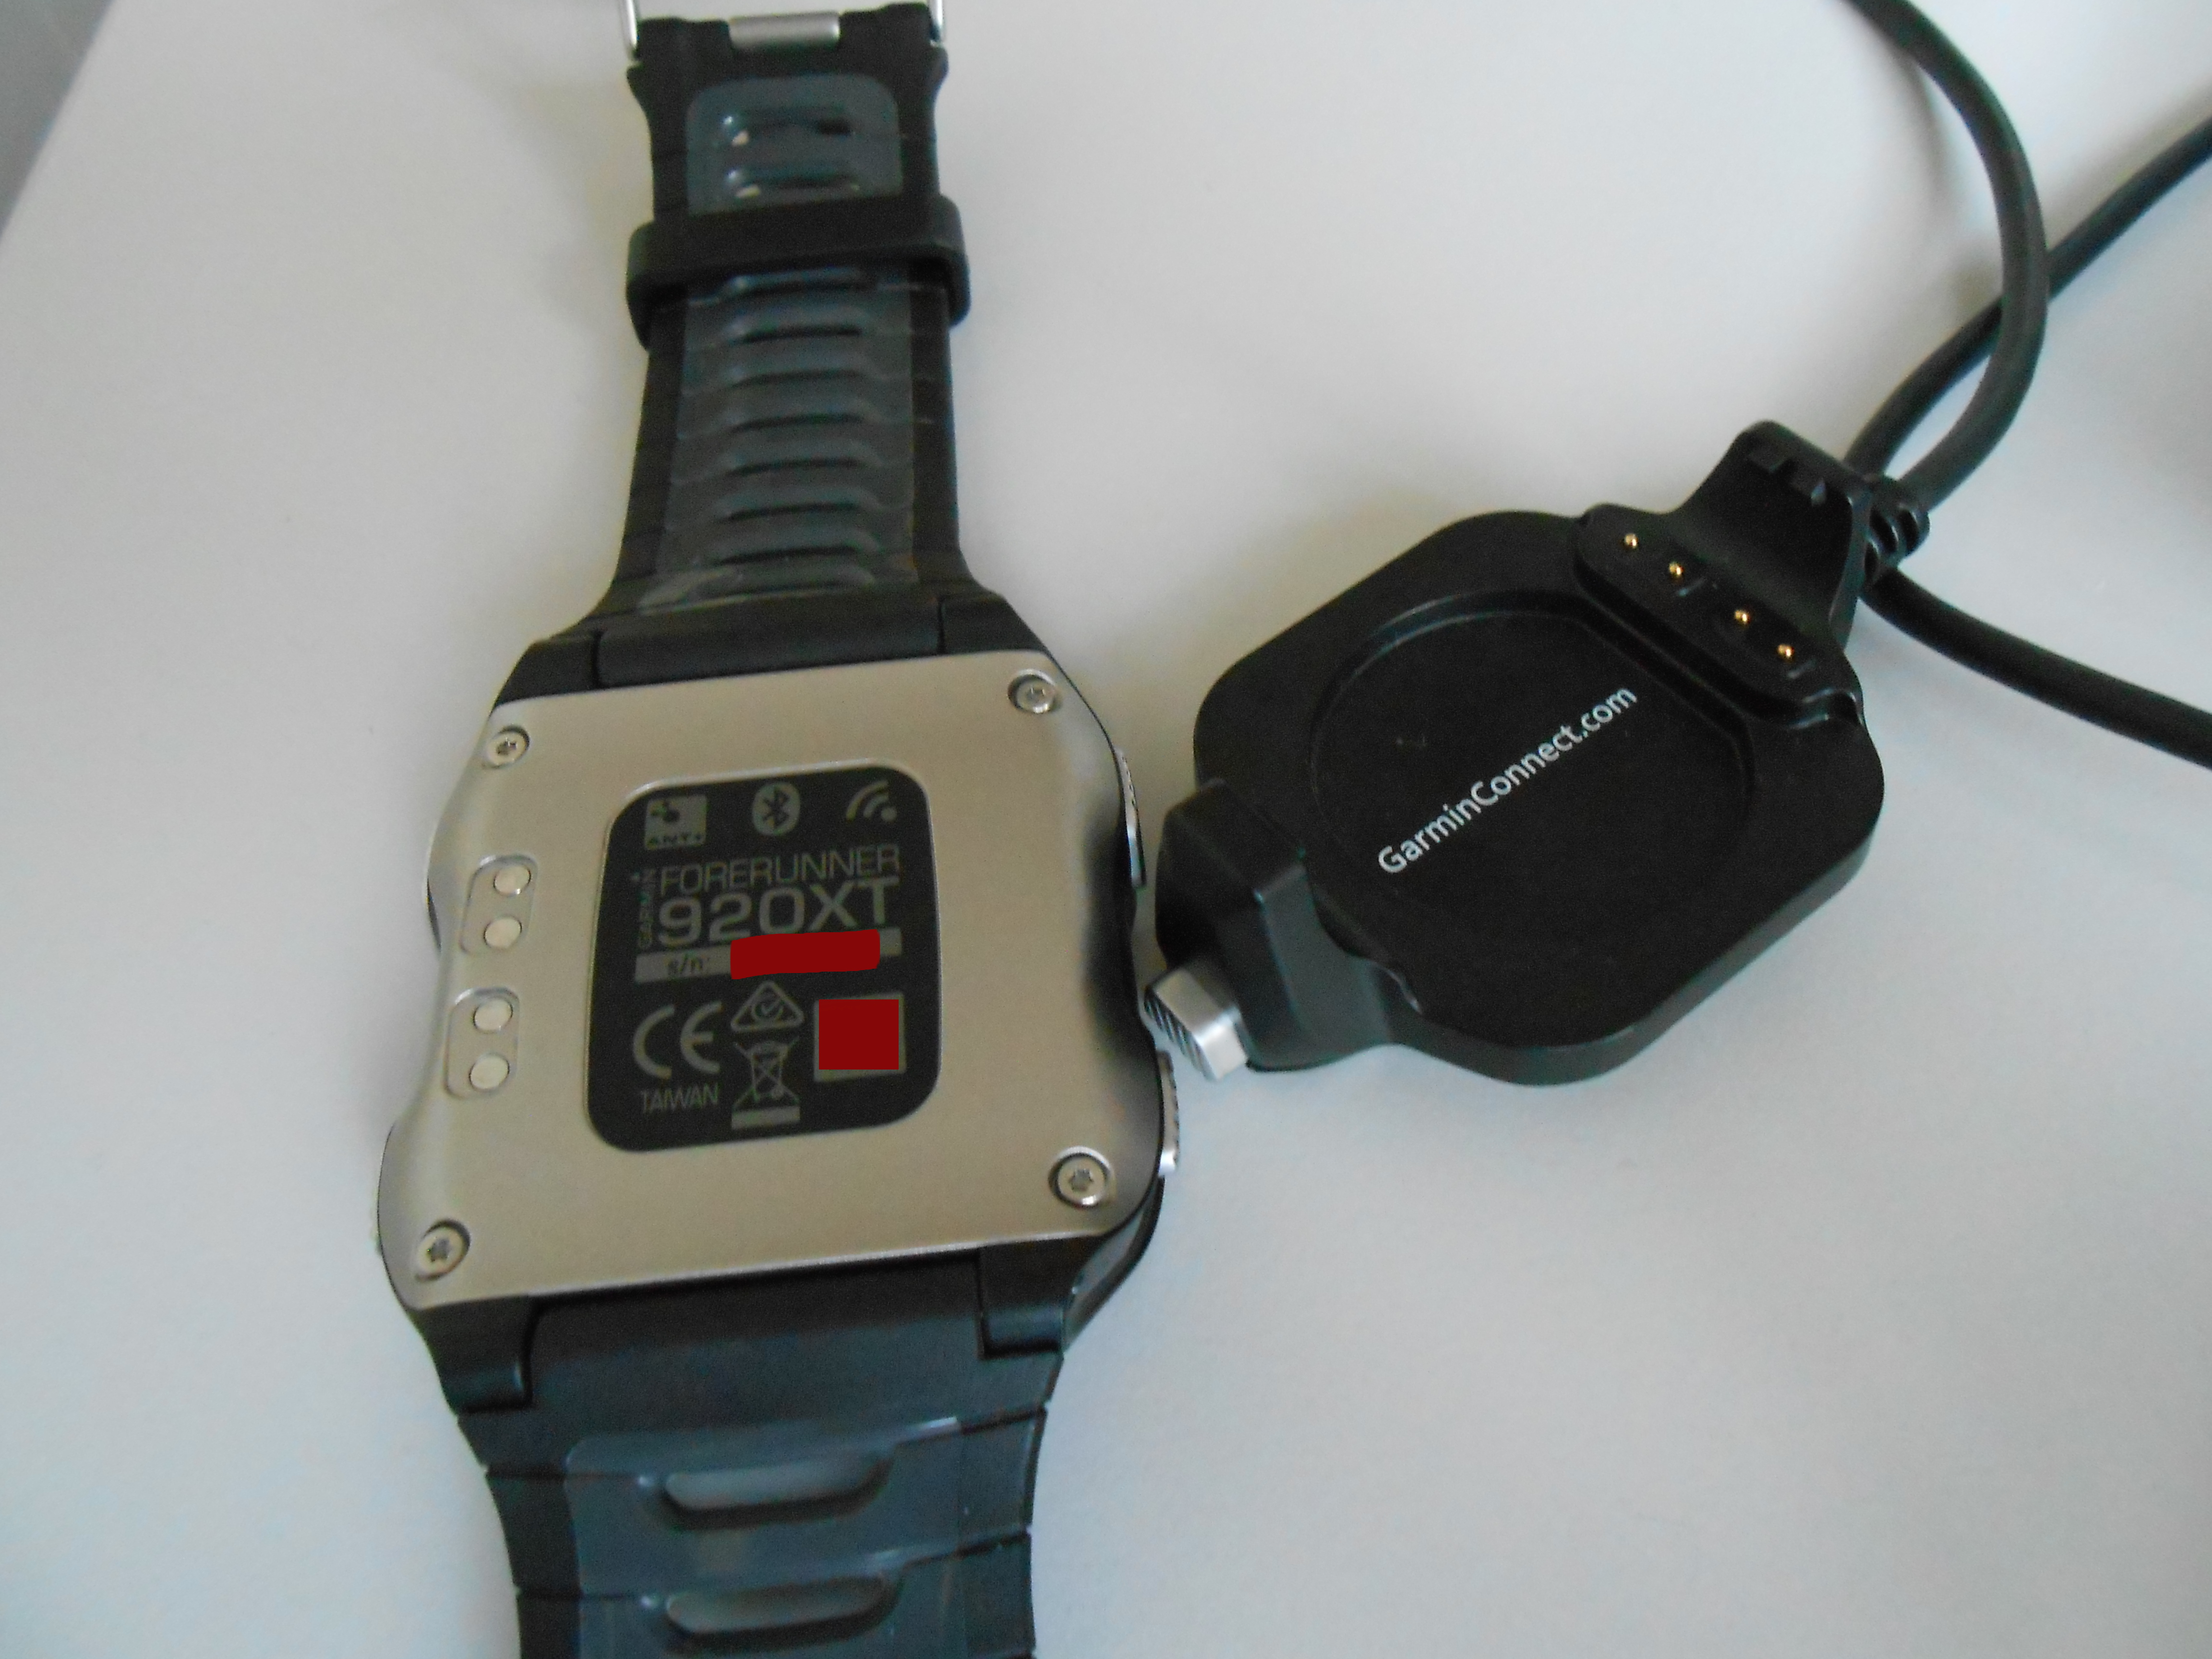
\includegraphics[width=.98\textwidth]{./forerunner_usb.JPG}
    \end{column}
    \begin{column}{.5\textwidth}
      \only<1>{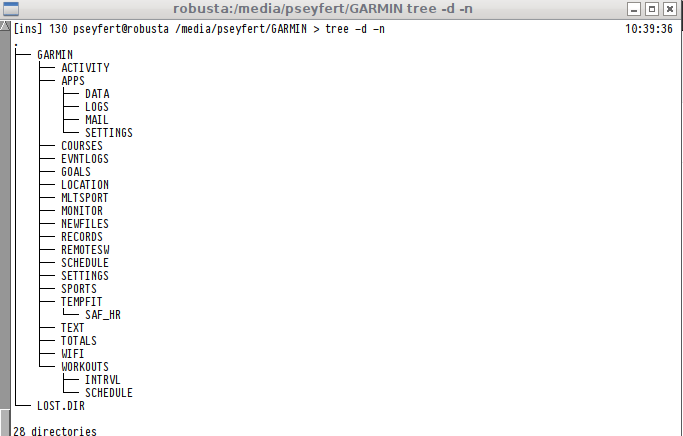
\includegraphics[width=.98\textwidth]{./fs.png}}
      \only<2>{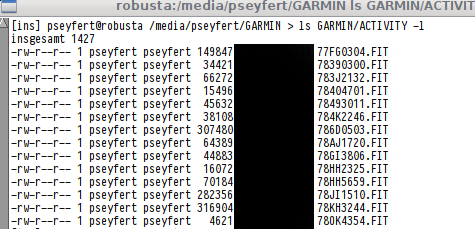
\includegraphics[width=.98\textwidth]{./activities.png}}
    \end{column}
  \end{columns}
\end{frame}

\begin{frame}
  \frametitle{modus operandi}
  \begin{itemize}
    \item fit files are (afaik) an open standard
    \item parsers and helpers are around
      \begin{itemize}
        \item gpsbabel
        \item python-fitparse / fitdump
        \item FIT-TO-TCX
      \end{itemize}
  \end{itemize}
  \begin{exampleblock}{my favourite: fitdump}
    \begin{itemize}
      \item dumps \emph{all} content of a fit file to the command line
      \item a few 100k lines for my largest files so far
      \item great point to start bodging
    \end{itemize}
  \end{exampleblock}
\end{frame}

\begin{frame}[t]
  \frametitle{dump}
  \only<1>{ 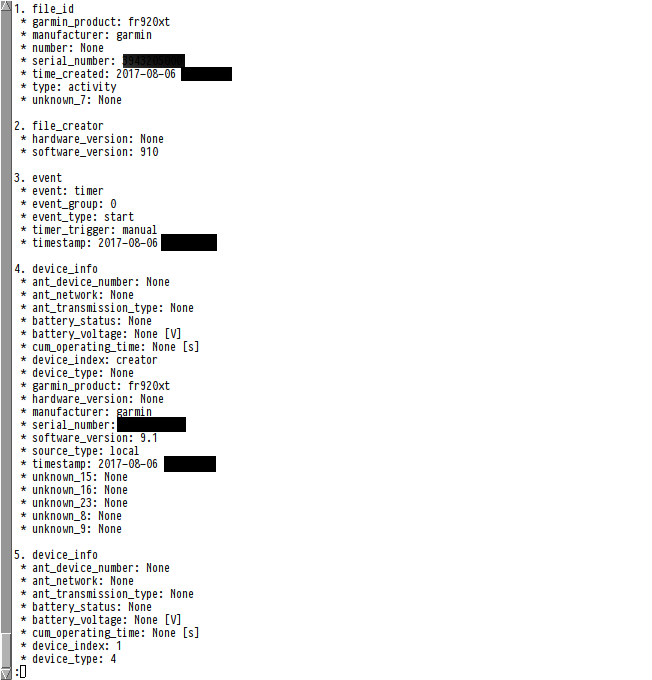
\includegraphics[width=.325\textwidth]{./bigdump1_.png}}
  \only<1>{ 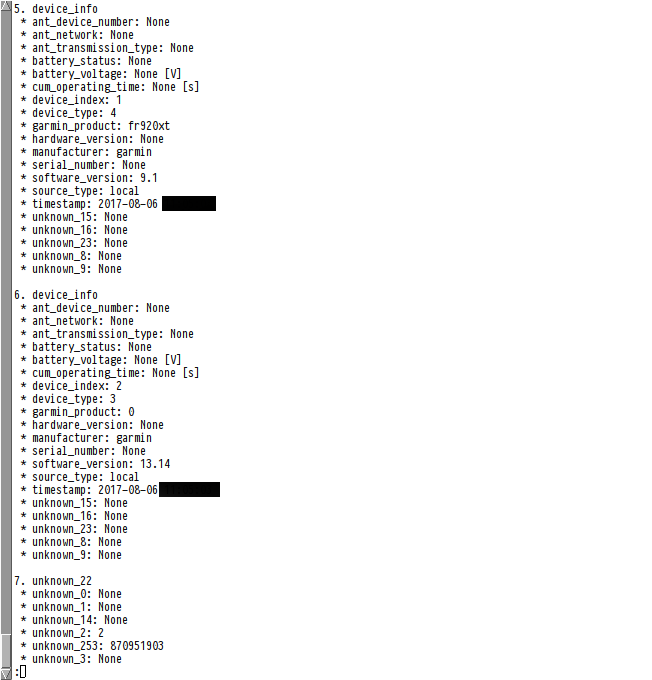
\includegraphics[width=.325\textwidth]{./bigdump2_.png}}
  \only<1>{ 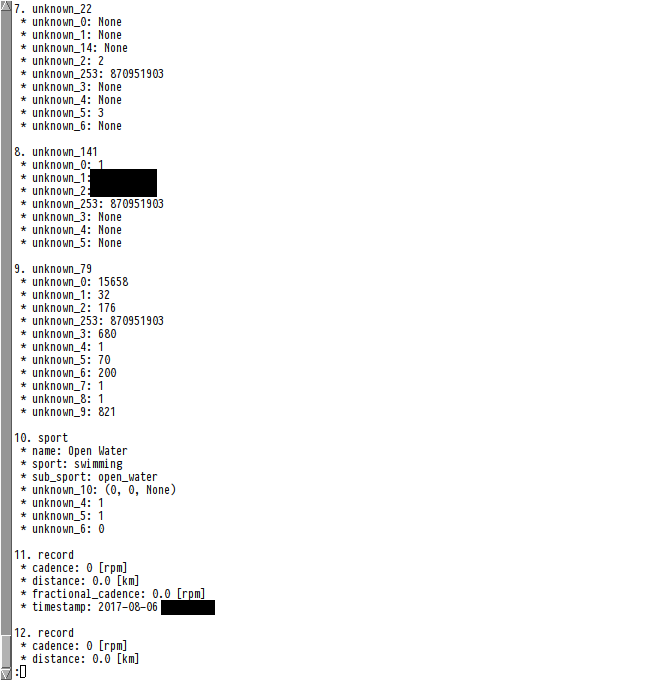
\includegraphics[width=.325\textwidth]{./bigdump3_.png}}
  \only<1>{ 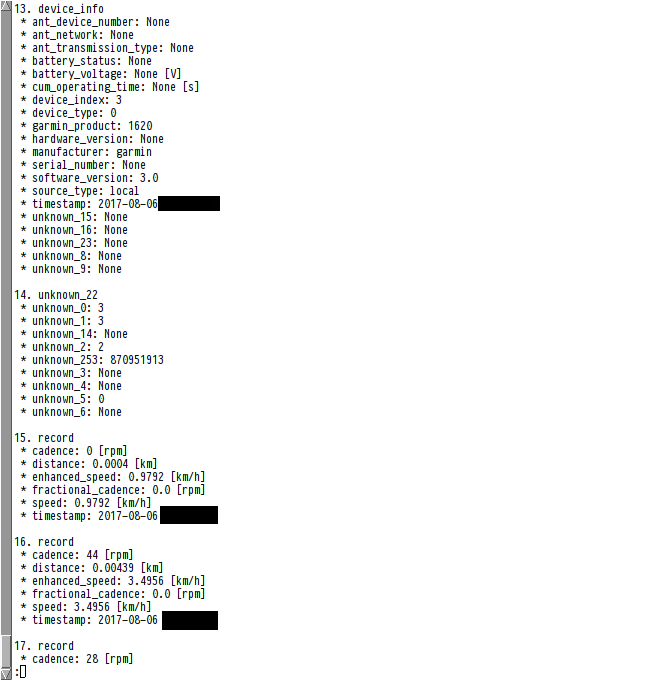
\includegraphics[width=.325\textwidth]{./bigdump4_.png}}
  \only<1>{ 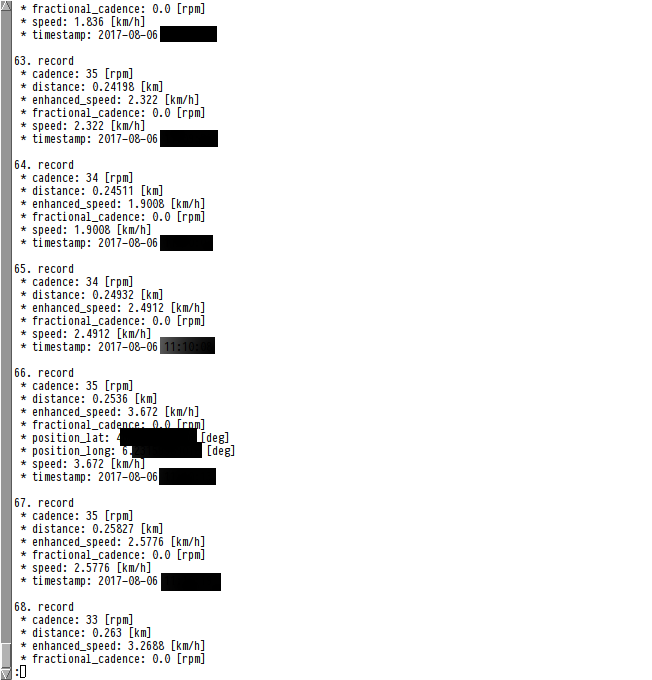
\includegraphics[width=.325\textwidth]{./bigdump5_.png}}
  \only<1>{ 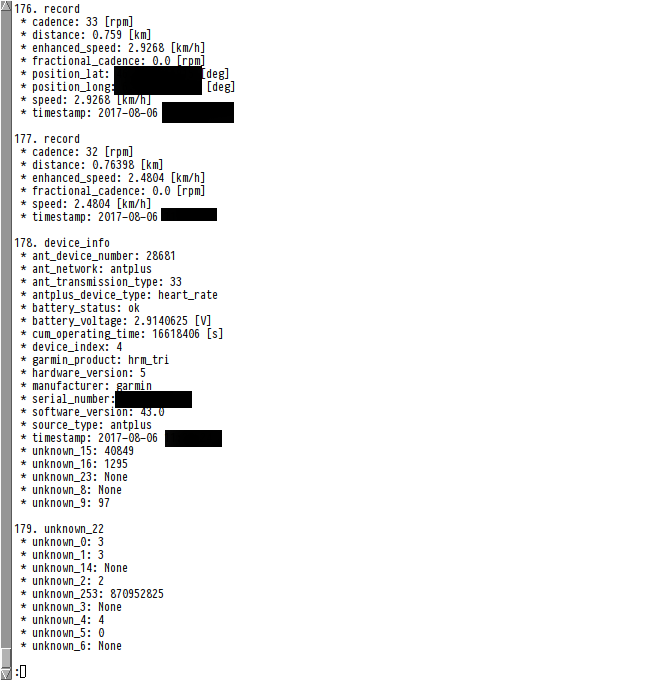
\includegraphics[width=.325\textwidth]{./bigdump6_.png}}
  \only<2>{ 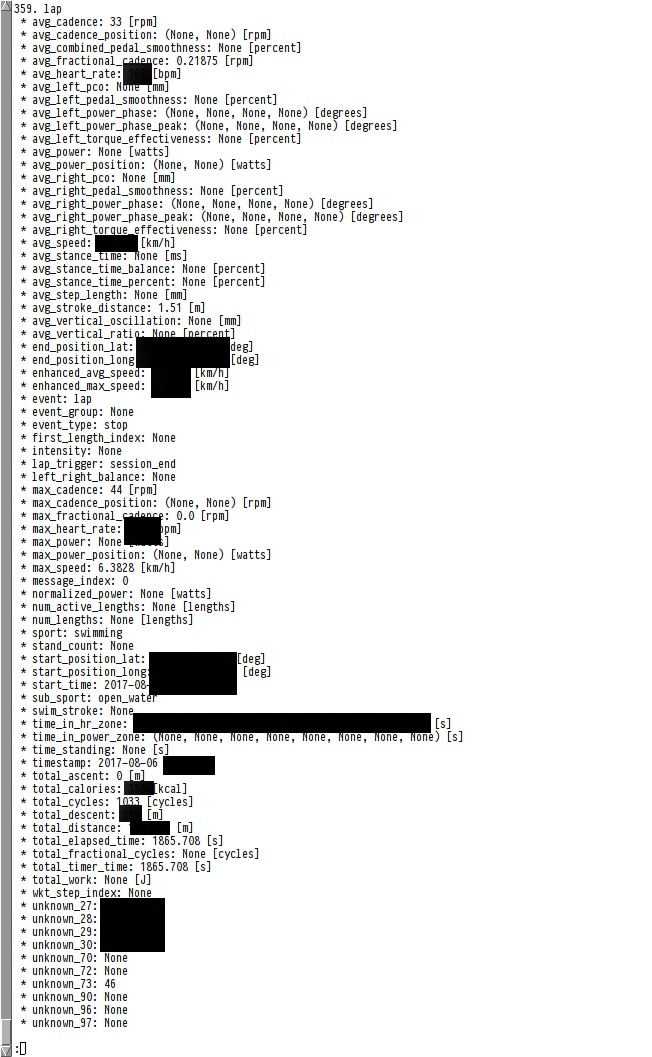
\includegraphics[width=.40\textwidth]{./bigdump7_.png}}
  \only<2>{ 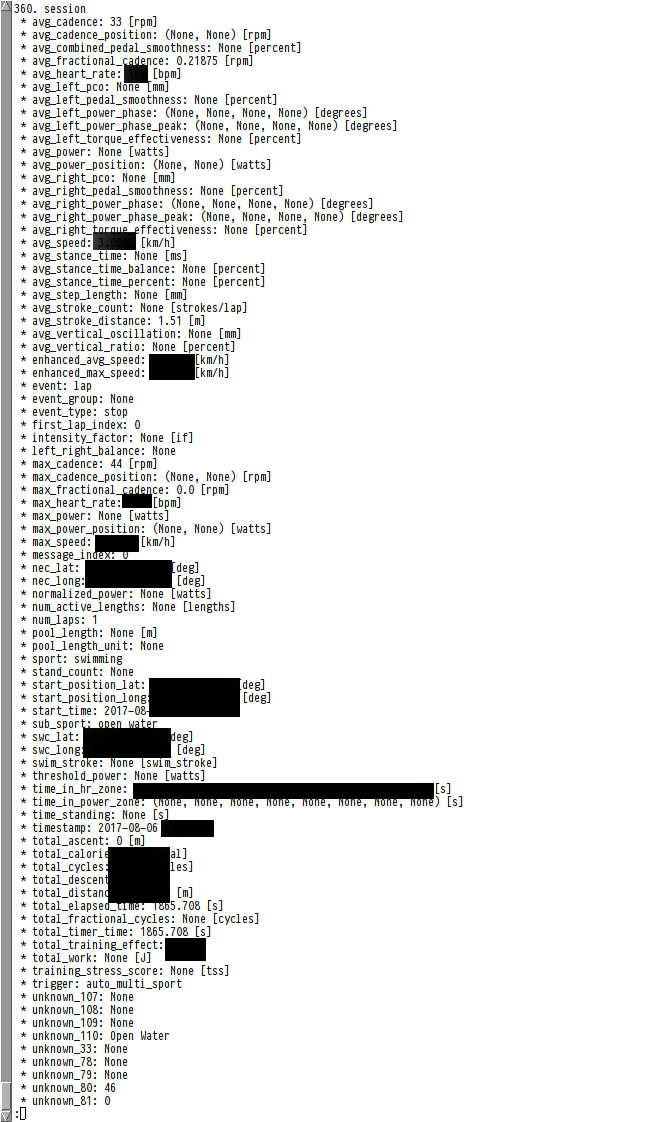
\includegraphics[width=.40\textwidth]{./bigdump8_.png}}
  \only<3>{ 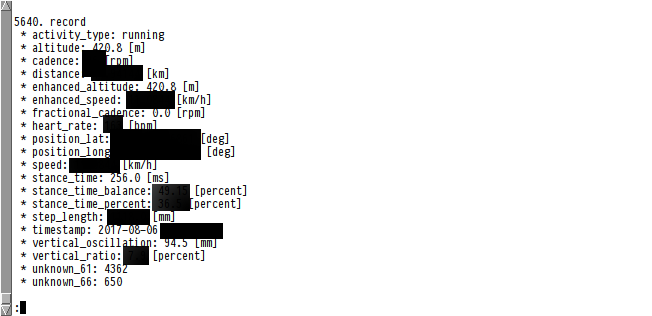
\includegraphics[width=.40\textwidth]{./bigdump9_.png}}
  \only<3>{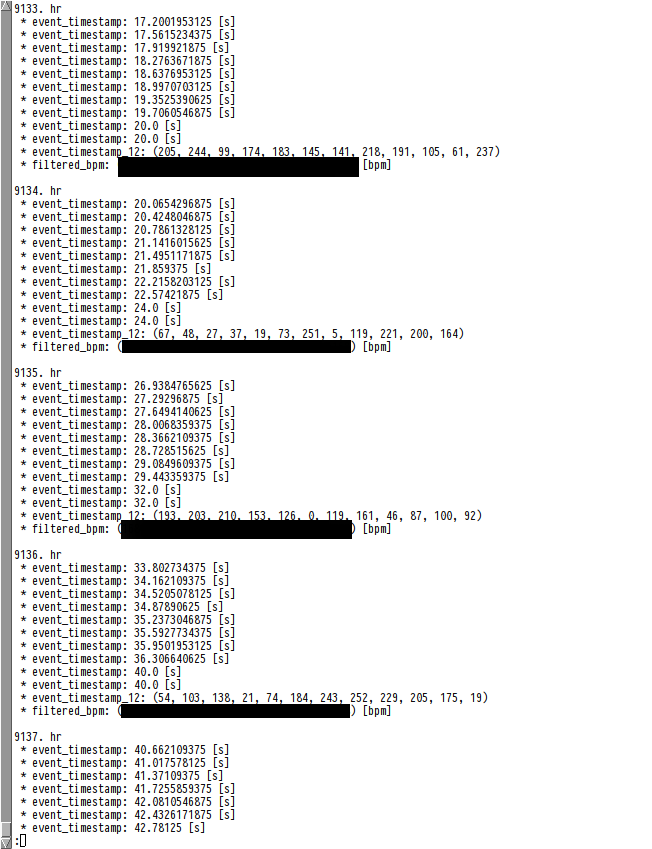
\includegraphics[width=.40\textwidth]{./bigdump10_.png}}
\end{frame}

\section[the inevitable problem avalanche]{the inevitable problem avalanche that was hiding behind the solution}
\begin{frame}
  \frametitle{problems \dots}
  \begin{columns}
    \begin{column}{.5\textwidth}
      \only<1>{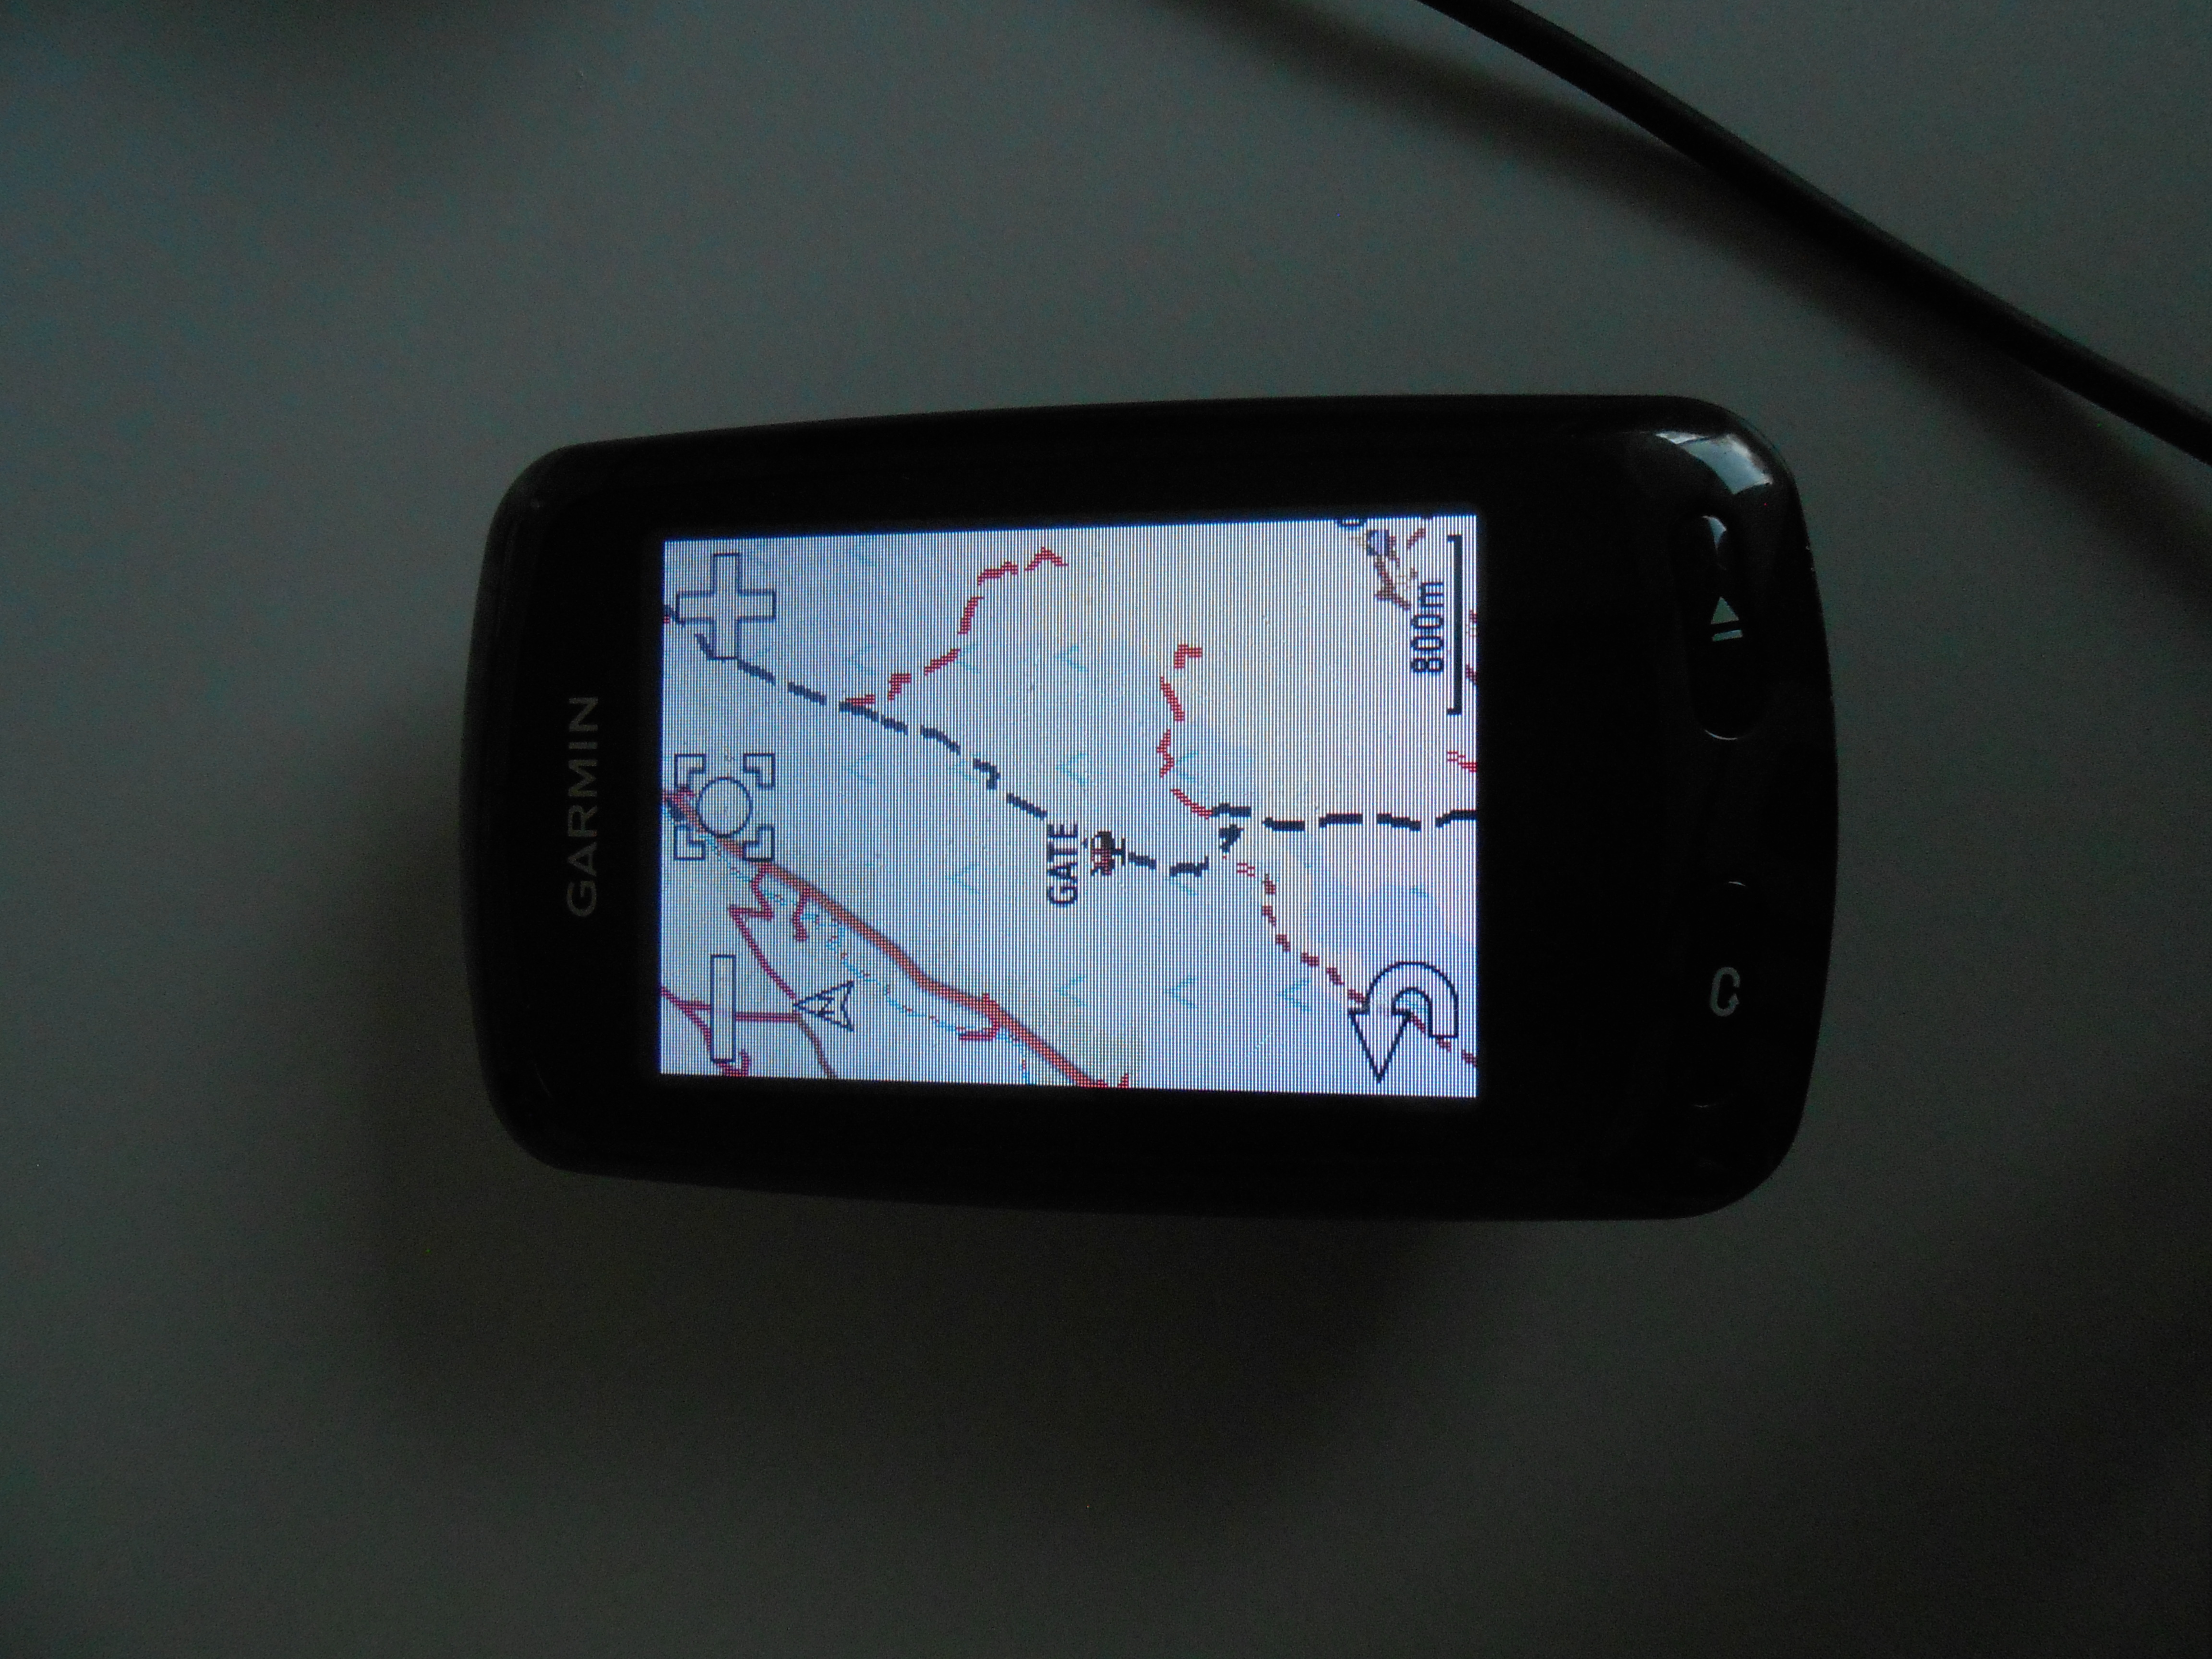
\includegraphics[width=\textwidth,angle =-90]{./DSCN5458.JPG}}
      \only<2>{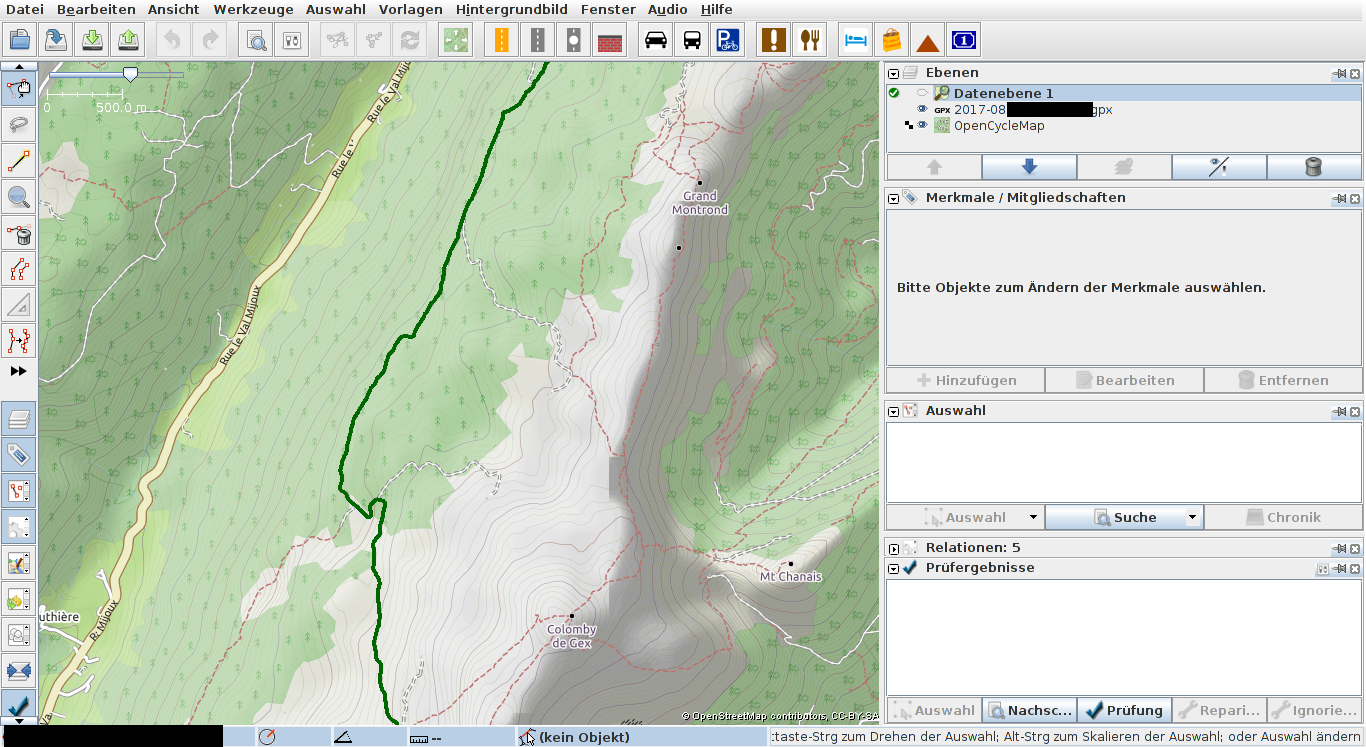
\includegraphics[width=\textwidth,angle = 00]{./josm_.png}}
      \only<3>{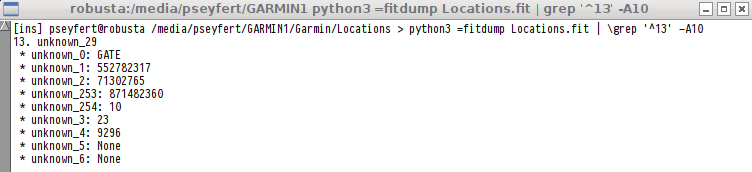
\includegraphics[width=\textwidth,angle = 00]{./locationdump.png}}
      \only<4>{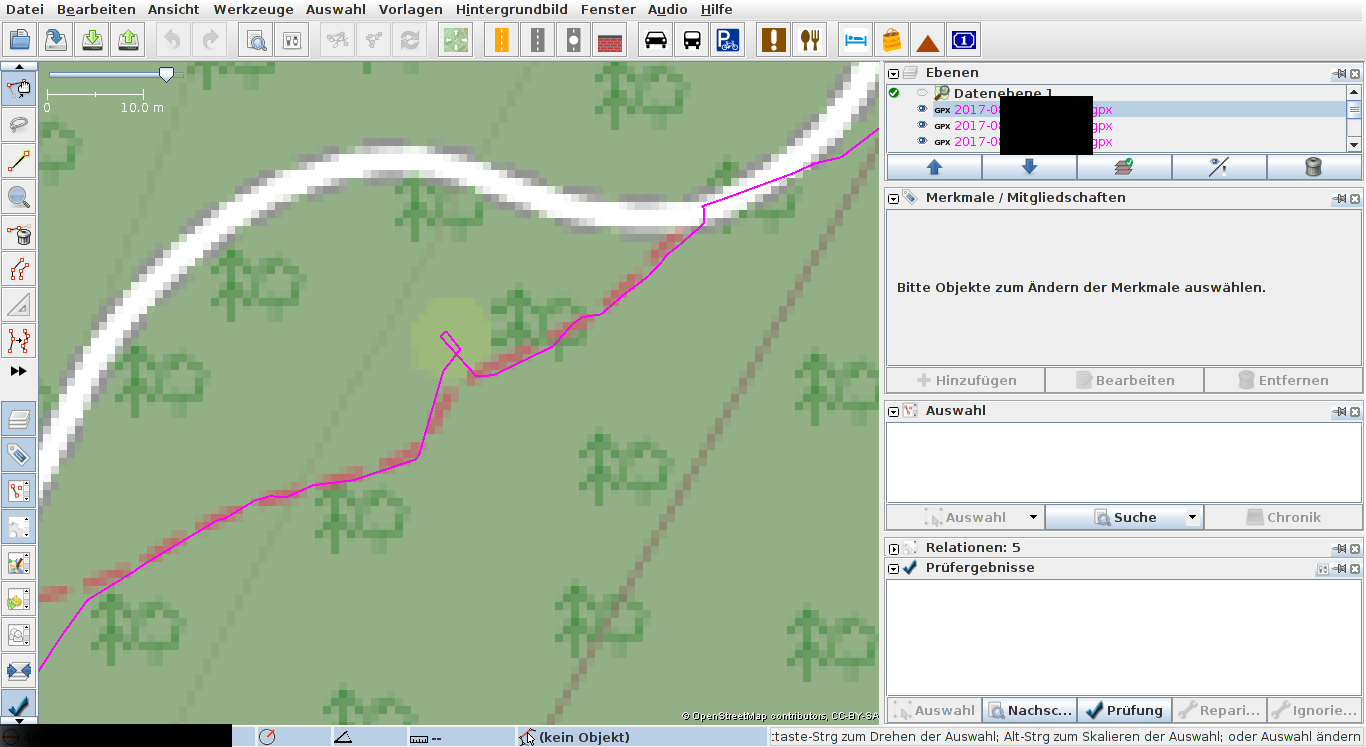
\includegraphics[width=\textwidth,angle = 00]{./loop_.png}}
    \end{column}
    \begin{column}{.5\textwidth}
      \begin{exampleblock}{locations}
        \begin{itemize}
            \item Can store locations when walking
              \newline $\rightarrow$ find point again
              \newline $\rightarrow$ add gate to OSM
            \item stored in {\tiny{\texttt{Garmin/Locations/Locations.fit}}}
        \end{itemize}
      \end{exampleblock}
      \begin{alertblock}{but\dots}
        \begin{itemize}
            \item<2-> not understood by gpsbabel
            \item<3-> not known to python-fitparse
            \item<4-> I don't want to walk in circles to mark positions on tracks
        \end{itemize}
      \end{alertblock}
    \end{column}
  \end{columns}
\end{frame}

\begin{frame}[t]
  \frametitle{problems \dots}
  \begin{columns}
    \begin{column}{.5\textwidth}
      \only<1->{
      \begin{itemize}
          \item heart rate is not recorded on the watch while swimming\newline (gets downladed at the end)
            \item and is dumped to the end of a fitfile
      \end{itemize}
    }
      \begin{alertblock}{}
        \begin{itemize}
            \item<2-> strange encoding of timestamps
            \item<2-> gets reset
            \item<2-> some ``extra data'' at the start
        \end{itemize}
      \end{alertblock}
  \end{column}
  \begin{column}{.5\textwidth}
    \only<1>{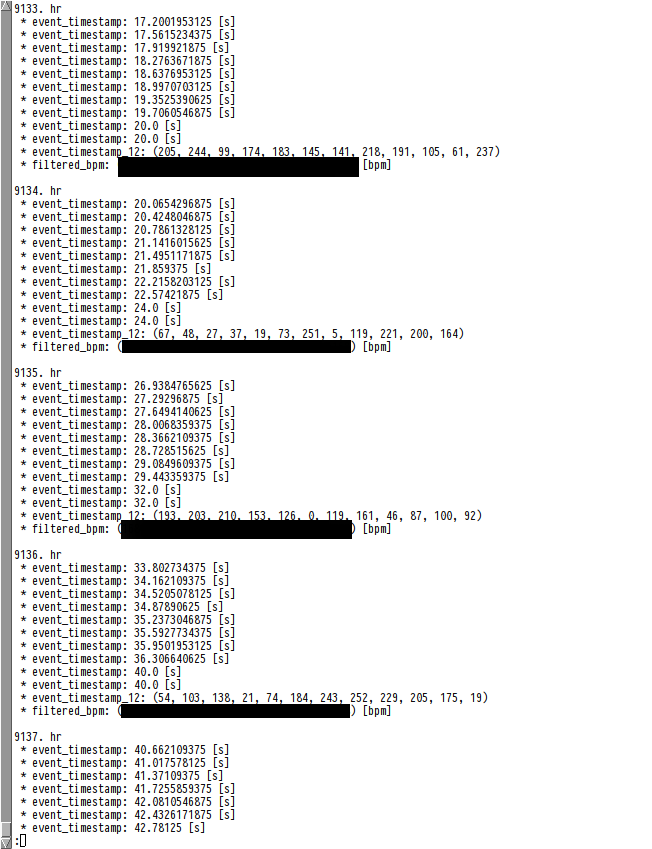
\includegraphics[width=\textwidth]{./bigdump10_.png}}
    \only<2>{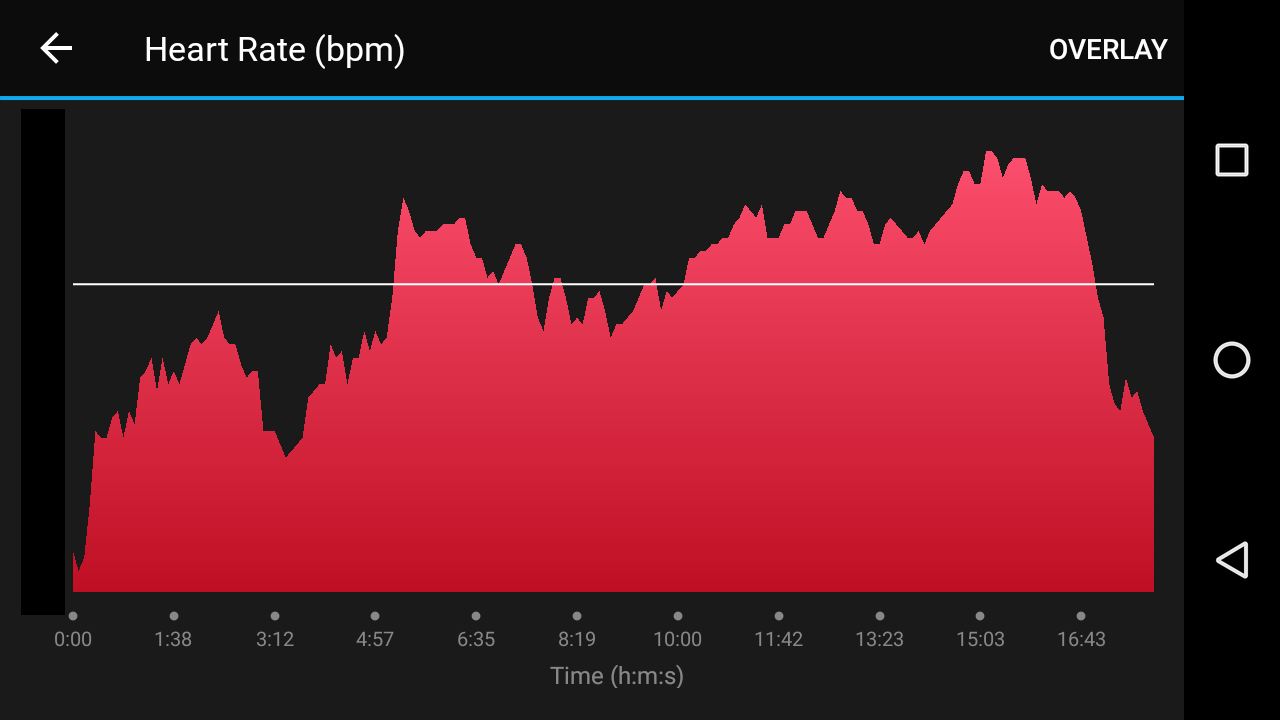
\includegraphics[width=\textwidth]{./swim_app_.png}\\
            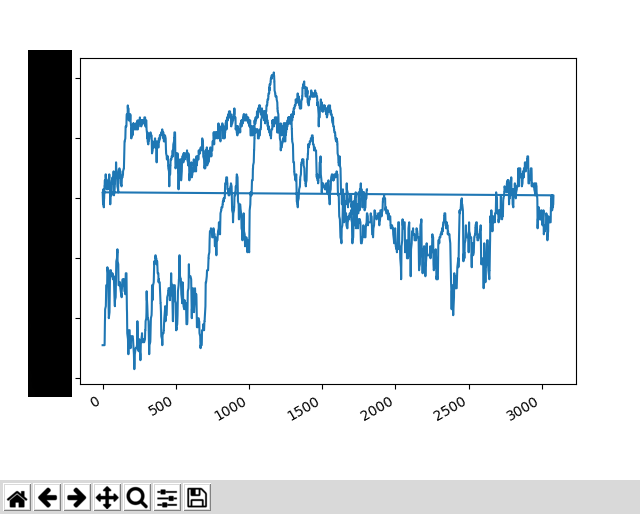
\includegraphics[width=\textwidth]{./swim_dump_.png}}
  \end{column}
  \end{columns}
\end{frame}

\begin{frame}
  \frametitle{limits of GPS}
  \begin{itemize}
      \item gpsbabel works reasonably well with most data
        \newline once one found the command line switches to include heart rate, temperature, \dots in the output
        \newline \texttt{gpsbabel -i garmin\_fit -f \$INPUTFILE -o gpx,gpxver=1.1,garminextensions -F \$OUTPUTFILE}
        \item but fails for records before GPS fix is established
          \newline (record of heart rate, speed, cadence, \dots is available in fitfile)
        \newline affects
        \begin{itemize}
            \item running
            \item cycling
            \item all indoor sports
        \end{itemize}
      \item \shrug okay for mapping/location related data mining
  \end{itemize}
\end{frame}

\section{join {fitfile-jugglers} on github!}
\begin{frame}
  \frametitle{what \myhref{https://github.com/pseyfert/fitfile-jugglers}{fitfile-jugglers} is about}
  \begin{block}{I want to}
    \begin{itemize}
    \item nerd around with my garmin data w/o the need of a smartphone or garmin's app or the cloud
    \item develop patches for python-fitparse, gpxpy, gpsbabel to understand more of the data garmin's devices record
    \item collect example code to analyse your own data
    \end{itemize}
  \end{block}
  \begin{exampleblock}{what's there}
    \only<1>{
      \begin{columns}
        \begin{column}{.48\textwidth}
      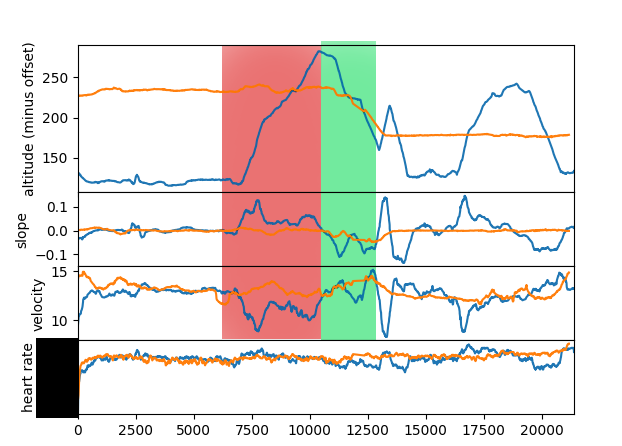
\includegraphics[width=.8\textwidth]{./HM.png}
        \end{column}
        \begin{column}{.48\textwidth}
          \begin{itemize}
              \item uphill I run slower than downhill!
          \end{itemize}
        \end{column}
        \end{columns}
    }
    \only<2-3>{
      \begin{columns}
        \begin{column}{.48\textwidth}
          \only<2>{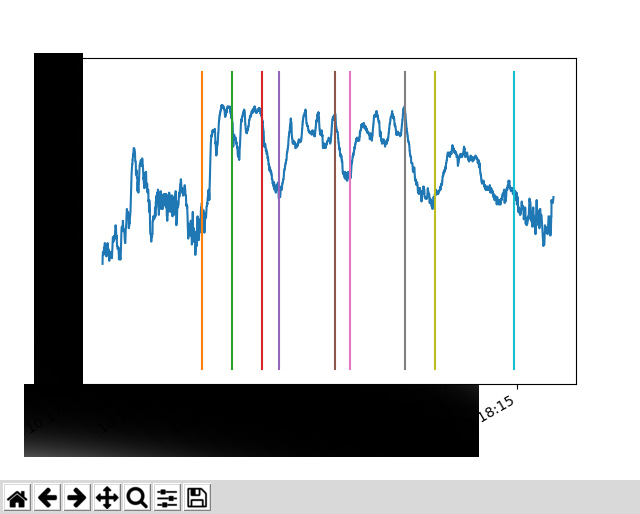
\includegraphics[width=\textwidth]{./hiit_.png}}
          \only<3>{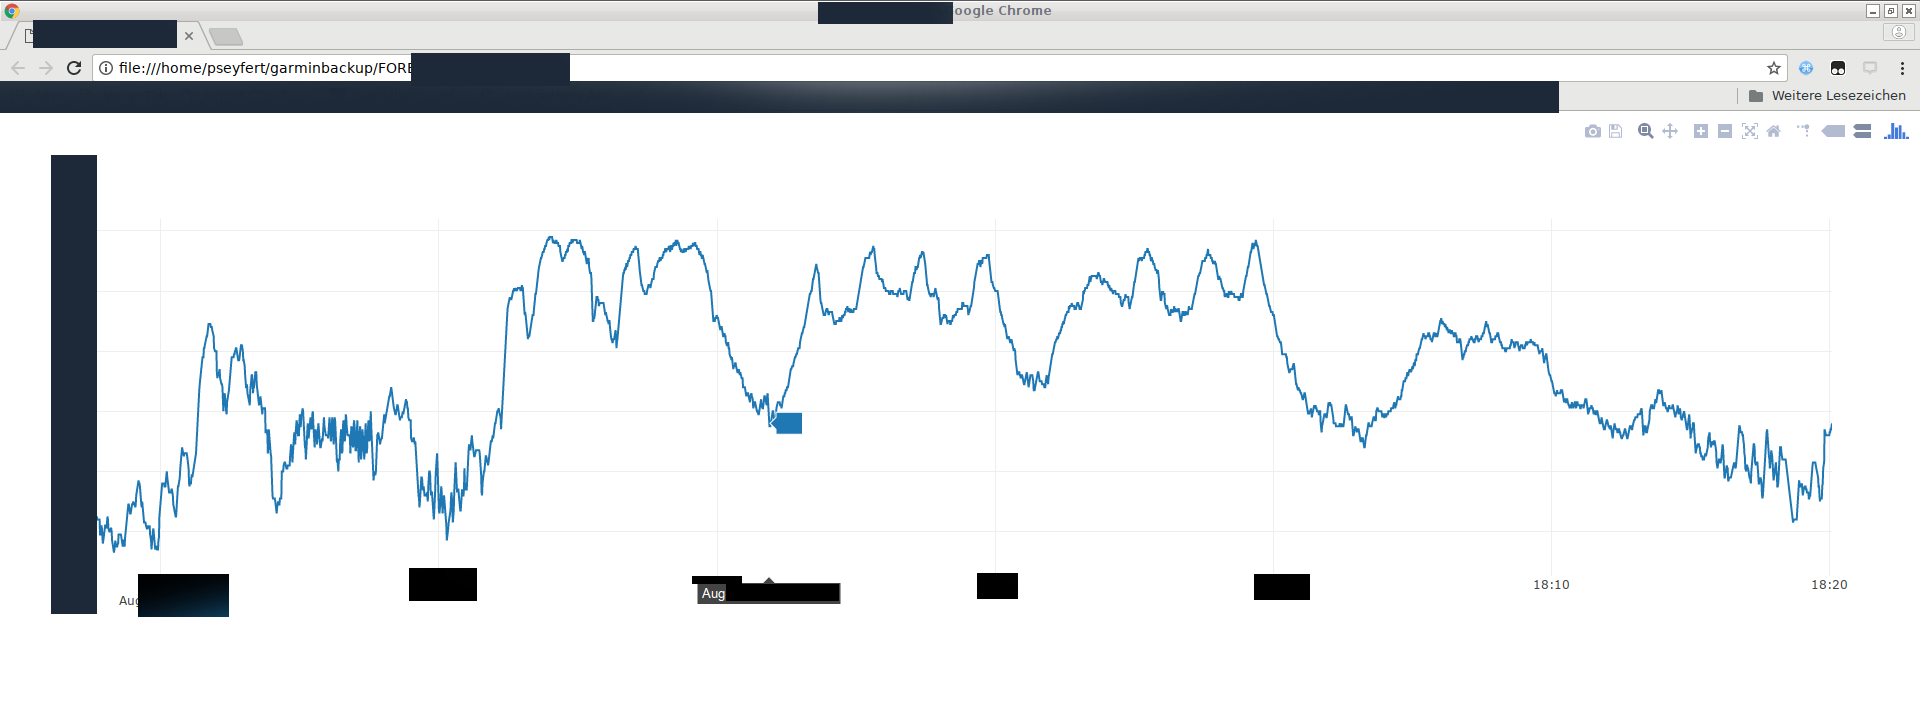
\includegraphics[width=\textwidth]{./hiit_browse.png}}
        \end{column}
        \begin{column}{.48\textwidth}
          \begin{itemize}
              \item plotting gps less, time stamped data
                \item<3> making html+javascript pages
                  \newline (if you need to show your friends on a smartphone)
          \end{itemize}
        \end{column}
        \end{columns}
    }
  \end{exampleblock}
\end{frame}

\begin{frame}
  
\includegraphics[width=.35\textwidth]{./QR.png}

  \texttt{https://github.com/pseyfert/fitfile-jugglers}
\end{frame}

\end{document}
